\begin{figure}[ht!]
	\centering
	\footnotesize

	\psfrag{b0}[l][c] {$\displaystyle \beta = \frac{0\pi}{6} = 0$}
	\psfrag{b1}[l][c] {$\displaystyle \beta = \frac{1\pi}{6}$}
	\psfrag{b2}[l][c] {$\displaystyle \beta = \frac{2\pi}{6} = \frac{\pi}{3}$}
	\psfrag{b3}[l][c] {$\displaystyle \beta = \frac{3\pi}{6} = \frac{\pi}{2}$}
	\psfrag{b4}[l][c] {$\displaystyle \beta = \frac{4\pi}{6} = \frac{2\pi}{3}$}
	\psfrag{b5}[l][c] {$\displaystyle \beta = \frac{5\pi}{6}$}
	\psfrag{b6}[l][c] {$\displaystyle \beta = \frac{6\pi}{6} = \pi$}

	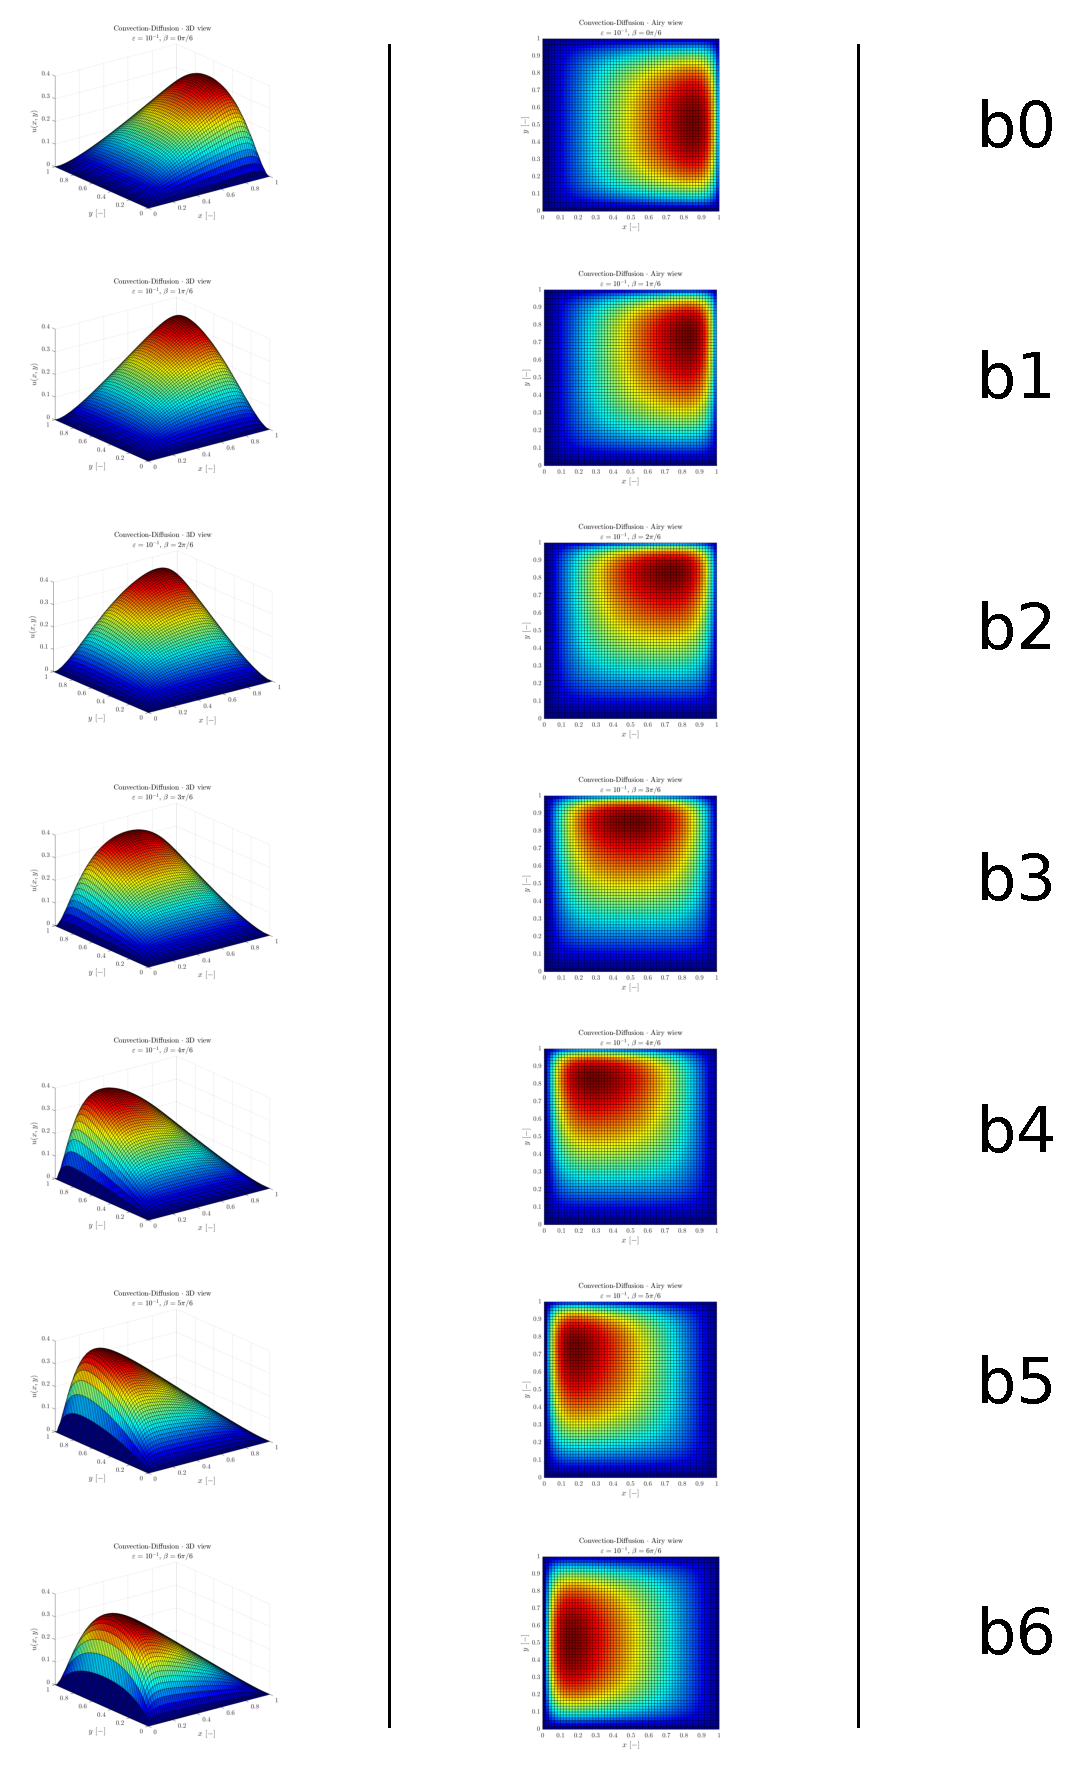
\includegraphics[width=0.85\textwidth]{fixedUpwind_variatedBeta.eps}
	\caption{Comparison among different values of
		$\displaystyle \beta = \left[0, \frac{\pi}{6}, \frac{2\pi}{6}, \frac{3\pi}{6}, \frac{4\pi}{6}, \frac{5\pi}{6}, \pi\right]$:
		Upwind differences used for discretizing convection terms $\partial_{x}u$ and $\partial_{y}u$;
		fixed $\varepsilon = 10^{-1}$.}
	\label{\LABEL}
\end{figure}